\documentclass[serif,mathserif]{beamer}
\usepackage{etex}
\usepackage{amsmath, amsfonts, epsfig, xspace}
\usepackage{algorithm,algorithmic}
\usepackage{pstricks,pst-node}
\usepackage{multimedia}
\usepackage[normal,tight,center]{subfigure}
\usepackage{beamerthemesplit}
\usepackage{color}

\setlength{\subfigcapskip}{-.5em}
\usetheme{lankton-keynote}

\usepackage{graphicx,color}
% remove caption of figure
\usepackage[labelformat=empty]{caption}

\usepackage[none]{hyphenat} % hyphenation is ugly in slides
\usepackage{parskip}

\usepackage{relsize} % \smaller to change size

\usepackage{tikz}
\usetikzlibrary{calc}

\usetikzlibrary{arrows}

\newcommand{\TikzDraw}[2][]{
  \begin{tikzpicture}[overlay, remember picture, shift={(current page.center)}, #1]
    #2
  \end{tikzpicture}
}

\newcommand{\gridlines}{
  \TikzDraw{
    \draw[help lines,xstep=.2,ystep=.2,red!20] (current page.south west) grid (current page.north east);
    \draw[help lines,xstep=1,ystep=1,red] (current page.south west) grid (current page.north east);
    \foreach \x in {-15,-14,...,15} {
      \node [anchor=north, red] at (\x,0) {\tiny \x};
      \node [anchor=east,red] at (0,\x) {\tiny \x};
    }
  }
}

\newcommand{\DrawOnImg}[3][]
{
  \begin{tikzpicture}
    \node[anchor=south west,inner sep=0] (image) at (0,0){
      #2
    };
    \begin{scope}[x={(image.south east)},y={(image.north west)}]
      \ifthenelse{\equal{#1}{grid}}
                 {\draw[color=blue, style=dashed] (0,0) grid[xstep=.1, ystep=.1] (1.0001,1.0001);}
                 {}
                 #3
    \end{scope}
  \end{tikzpicture}
}


\author[Jiong Chen]{Jiong Chen}

\title[\hspace{2em}\insertframenumber/\inserttotalframenumber]{Large-Scale Bounded Distortion Mappings}

\date{October 28, 2015} %leave out for today's date to be insterted

% \institute{Zhejiang University}

\newcommand{\BOLD}[1]{\mathbf{#1}}
\newcommand{\PDIF}[2]{\frac{\partial #1}{\partial #2}}
\newcommand{\TODO}[1]{\textcolor{red}{#1}}
\DeclareMathOperator{\tr}{tr}
\DeclareMathOperator{\cond}{cond}
\DeclareMathOperator{\ST}{s.t.}

\definecolor{DARK}{RGB}{45, 33, 73}
\definecolor{LIGHT}{RGB}{119, 52, 106}
\definecolor{TEXTLIGHT}{RGB}{213, 207, 229}
\definecolor{TEXTDARK}{RGB}{66, 66, 66}
\definecolor{BULLET}{RGB}{179, 17, 102}
\definecolor{EM}{RGB}{179,17,102}

\begin{document}

\maketitle

\begin{frame}
 \frametitle{Problem statement}
 \begin{itemize}
  \item Given an initial map, compute a similar map whose differentials are \TODO{orientation preserving}
  and have \TODO{bounded condition number}.
  \Large
 \begin{equation*}
 \boxed{
  \begin{aligned}
    \min_{\BOLD{x}}~~&\|T\BOLD{x}-T\BOLD{x}_0\|_2  \\ 
    \ST \quad &A\BOLD{x} = \BOLD{b}\\
    &T_j\BOLD{x} \in \mathcal{D}_j
  \end{aligned}
 }
 \end{equation*}
 \large
 \item $\mathcal{D}_j=\mathcal{D}^K, j=1,2,\dots m$
 \begin{equation*}
  \det(D^K) \ge  0, \quad \cond(D^K) \le K
 \end{equation*}
 \end{itemize}
\end{frame}

\begin{frame}
 \frametitle{Problems statement}
 \begin{itemize}
  \item Nonlinear bounded distortion constraints $\Rightarrow$ difficult \& computationally demanding
  \item Numerical methods: first-order \& second order
  \item Second order: interior point solver \& Newton variants
  \item First order 
    \begin{itemize}
     \item[-] \textcolor{red}{Alternating optimization\,(Local/global, block descent)}
     \item[-] \textcolor{green!50!black}{Gauss-Newton for least squares}
    \end{itemize}
 \end{itemize}
\end{frame}

\begin{frame}
 \frametitle{Approach}
\end{frame}

\begin{frame}
 \frametitle{Algorithmic details}
\end{frame}


\begin{frame}
 \frametitle{Evaluation: performance}
 \begin{figure}
  \centering
  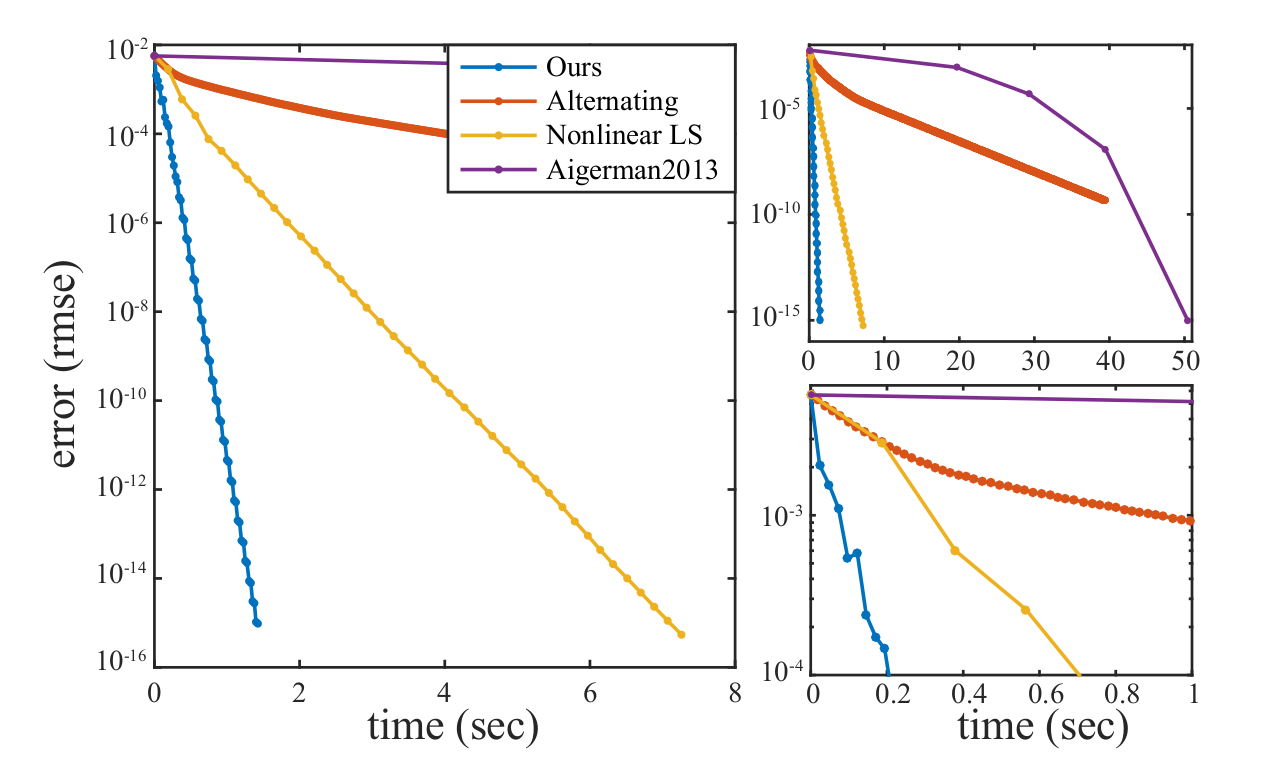
\includegraphics[width=10cm, height=5cm]{img/performance.png}
 \end{figure}
\end{frame}

\begin{frame}
 \frametitle{Evaluation: scalability}
 \begin{figure}[t]
  \centering  
  \begin{minipage}[t][0.9\textheight][s]{1\textwidth}
    \centering
    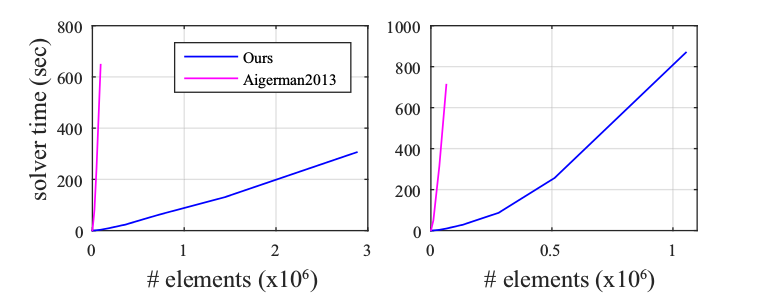
\includegraphics[scale=0.35]{img/sc0.png} 
    \vfill
    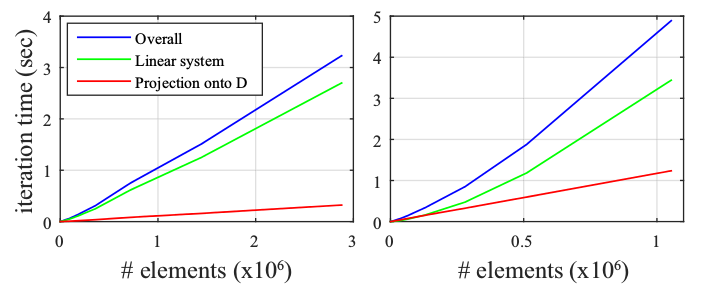
\includegraphics[scale=0.35]{img/sc1.png}
  \end{minipage}
 \end{figure}
\end{frame}

\begin{frame}
 \frametitle{Evaluation: robustness}
 \begin{figure}[t]
  \centering
  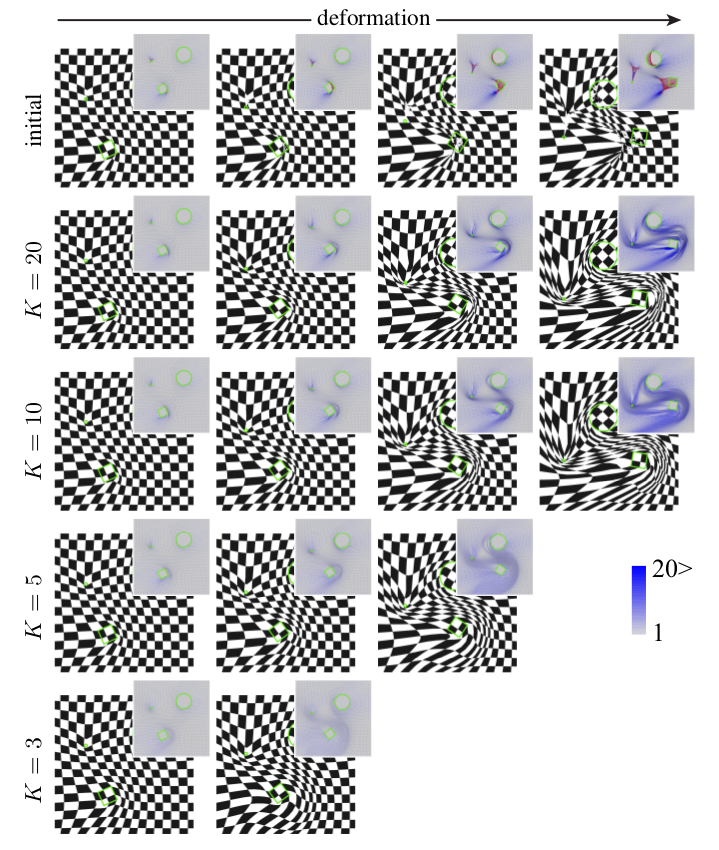
\includegraphics[width=9cm, height=8cm]{img/robustness.png}
 \end{figure}
\end{frame}

\begin{frame}
 \frametitle{More examples}
\end{frame}

\begin{frame}
 \frametitle{Conclusion}
 \begin{itemize}
  \item Pros:
    \begin{itemize}
      \item[-] Key: single linear hyperplane $\overset{\text{local}}{\approx}$ set of BD maps
      \item[-] Comparable computational efficiency to that of alternating optimization
      \item[-] improved convergence properties 
    \end{itemize}
  \item Cons:
    \begin{itemize}
      \item[-] Lacks global convergence guarantees
      \item[-] Limited to mappings satisfying bounds on distortion
  \end{itemize}
 \end{itemize}
\end{frame}

\begin{frame} 
  \TikzDraw {
    \node at (0, 0.5) {\Huge{Thanks!}};
  }
  %\gridlines
\end{frame}


\end{document}
